% XCircuit output "eprom.tex" for LaTeX input from eprom.eps
\def\putbox#1#2#3#4{\makebox[0in][l]{\makebox[#1][l]{}\raisebox{\baselineskip}[0in][0in]{\raisebox{#2}[0in][0in]{\scalebox{#3}{#4}}}}}
\def\rightbox#1{\makebox[0in][r]{#1}}
\def\centbox#1{\makebox[0in]{#1}}
\def\topbox#1{\raisebox{-0.60\baselineskip}[0in][0in]{#1}}
\def\midbox#1{\raisebox{-0.20\baselineskip}[0in][0in]{#1}}
\begin{center}
   \scalebox{0.6}{
   \normalsize
   \parbox{2.04688in}{
   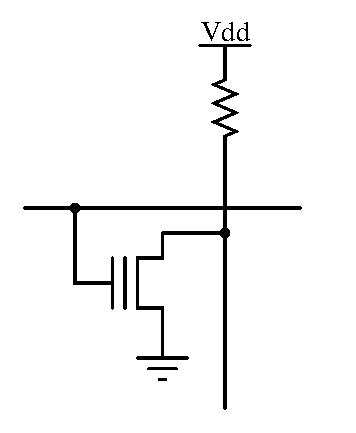
\includegraphics[scale=1]{memorie/eprom.eps}\\
   % translate x=608 y=256 scale 0.38
   \putbox{1.56in}{2.06in}{1.20}{$R_{PU}$}%
   } % close 'parbox'
   } % close 'scalebox'
   \vspace{-\baselineskip} % this is not necessary, but looks better
\end{center}
